\documentclass[usegeometry=true]{scrartcl}
\usepackage[ngerman]{babel}
\usepackage[T1]{fontenc}
\usepackage{lmodern}
\usepackage[utf8]{inputenc}
\usepackage{hyperref}
\usepackage{amssymb}
% Dimensionen bitte nicht ändern. 
\usepackage[left=2cm, right=2cm, top=2cm, bottom=2cm, bindingoffset=1cm, includeheadfoot]{geometry}
%Zeilenabstand bitte nicht ändern
\usepackage[onehalfspacing]{setspace}

%--- Wrap text around figures
\usepackage{wrapfig}

% --- Abkürzungsverzeichnis ---
\usepackage[nohyperlinks, 
withpage, 
smaller,
footnote
]{acronym}



% --- Grafiken ---
\usepackage{graphicx}
\usepackage{subfig}



\usepackage[backend=biber,style=numeric,]{biblatex}\addbibresource{Visualisierung.bib}

\begin{document}
\pagenumbering{Roman}

\begin{titlepage}
	\begin{center}
		\large{\textsc{Martin-Luther-Universität Halle-Wittenberg}}\\
				

		\setstretch{1.5}
		Projektbericht zum Modul Information Retrieval und Visualisierung Sommersemester 2021
	\end{center}

	\begin{center}
		\Large
		\textbf{Visualisierung von Daten des Videospiels Fifa 21}
	\end{center}

	\vskip 1cm

	\vskip 0.75cm

	\begin{center}
		\begin{tabular}{lll}
			Eingereicht bei:& & Dr. Alexander Hinneburg\\
			Eingereicht von:  & & Johannes Lange \\
			%& & Krukenbergstraße 9\\
			%& & 06112 Halle (Saale)\\
			& & \\
			Eingereicht am: & & \today
		\end{tabular}
	\end{center}

\end{titlepage}



% ----------------------------------------------------------------------------

\newpage
%----------------------------------------------------------------------------
% Inhaltsverzeichnis:
\tableofcontents
\newpage

% Abbildungsverzeichnis
\clearpage
\listoffigures

% Abkürzungsverzeichnis:
\section*{Abkürzungsverzeichnis}\label{AV}
	\addcontentsline{toc}{section}{Abkürzungsverzeichnis}
	\begin{acronym}
	\acro{FUT}[FUT]{Fifa Ultimate Team}
	\end{acronym}
\newpage
% ----------------------------------------------------------------------------
% Gliederung und Text:
\pagenumbering{arabic}
\section{Einleitung}

% -Zu Parallel Koordinaten on Hover inklusive der verglichenen Werte hinzufügen
% -Aggregationsfunktion möglicherweise entfernen, überprüfen ob der Code deutlich schneller läuft
% -Torhüter herausfiltern, da diese keine Werte haben
% -Filter Funktion in parallelen Koordinaten und Scatterplot erweitern
%Tipps zu Latex und Koma-Script für Hausarbeiten sind im \href{http://mirrors.ctan.org/info/latex-refsheet/LaTeX_RefSheet.pdf}{LaTeX Reference Sheet for a thesis with KOMA-Script} von Marion Lammarsch und Elke Schubert zusammengefasst. 
%Der Bericht fällt in die Kategorie von InfoVis-Paper, die Tamara Munzner Design Study nennt \cite{Munzner2008}: In der Einleitung sollen sie zuerst das Zielproblem beschrieben. Daraus sollen sie Fragestellungen motivieren, die mittels Techniken der Informationsvisualisierung beantwortet werden können. 

%\textbf{Tamara Munzner angucken}\\
%\textbf{Zielprobelm formulieren und daraus Fragestellung schreiben -> Wie können diese mittels Visualisierung beantwortet werden}


Die Visualisierung von Daten nimmt mit Hinblick auf Big Data und damit immer unübersichtlicheren Datengrundlagen an Bedeutung zu. Um aus großen Mengen von Daten neue Informationen zu gewinnen reicht es nicht aus die Daten direkt zu analysieren. Durch die Anwendung der richtigen Visualisierungstechniken können neue Informationen gewonnen werden.\\
Besonders Fans von kompetetiven Videospielen versuchen oft jeden möglichen Vorteil zu nutzen um gewinnen zu können.
Das Spiel FIFA 21, dessen Daten in dieser Arbeit visualsiert werden, bildet dabei keine Ausnahme.
Früher wurden dazu häufig Guides verwendet in denen hunderte Seiten Tipps und Tricks abgedruckt worden sind. Diese Guides bieten jedoch keine Interaktion und sind oft aus der subjektiven Sicht eines Autors verfasst. 
Moderne Visualisierungstechniken erlauben es jedoch deutlich mehr Informationen zu extrahieren und für die Spieler interaktiv nutzbar zu machen.
Der gegebene Datensatz ist äußerst umfangreich, zu über 16000 Sportlern sind jeweils 107 Variablen festgehalten. Diese reichen von \textit{Name} über \textit{Verein} bis hin zu \textit{Schusskraft} eines Spielers.
Zwar sind diese Daten dem Videospiel FIFA 21 entnommen, Daten wie Name, Alter, Verein oder ähnliche beruhen aber auf echten Daten der Spieler. Weiterhin versucht der Hersteller des Spiels auch die restlichen Daten so nah an der Realität zu verankern wie möglich.
So besteht die Hoffnung mittels Visualisierungstechniken noch weitgreifendere Erkenntnisse aus dem gegebenen Datensatz ziehen zu können, als solche die Spielern des Spiels dienen.\\
Spieler des Spiels möchten möglicherweise herausfinden, welcher Fussballer ihr Team verbessert aber wenig kostet also: \textit{Welche Spieler hat das höchste Overall bei geringstem Gehalt?}\\
Eine Weitere Frage könnte sich beim Bau eines Teams bestehend aus Bundesliga Teams ergeben wenn noch ein Spieler einer bestimmten Position benötigt wird: \textit{Welche Linksverteidiger spielen in der Bundesliga?}\\
Außerdem könnten sich Fragen nach den besten Spielern bezüglich individueller Kriterien ergeben: \textit{Welcher Stürmer ist schnell, Schussstark, kann gut dribbeln und ist groß?}\\
Diese konkreten Fragen beziehen sich alle auf Fragen welche Anforderungen von Spielern des Spiels darstellen.\\
Ob Fragen von anderen Anforderungsgruppen, wie bspw. Sportwissenschaftlern beantwortet werden können: \textit{Wann erreichen Fussballer ihren Peak? Sind größere Fussballer besser, schneller, etc.?} ist dabei nicht klar, da alle nicht erhobenen Daten von Mitarbeitern des Herstellers festgelegt worden sind und somit nicht genau den tatsächlichen Daten entsprechen können. Trotzdem lohnt es sich dies zu überprüfen und mit anderen wissenschaftlichen Arbeiten abzugleichen.

\newpage


\subsection{Anwendungshintergrund}
%Sie müssen genug Hintergrund bereitstellen, so dass die Lesenden sich ein Urteil bilden können, ob ihre Lösung funktioniert. Sie sollen die Lesenden jedoch nicht mit Anwendungsdetails so überschütten, dass der Fokus auf die Fragen zur Informationsvisualisierung untergehen. 
%\textbf{Was sind die Daten, sind die Visualisierungslösungen angebracht, möglicherweise auf einzelne Variablen eingehen}\cite{Munzner2008}

Im folgenden werden die drei verwendeten Visualisierungstechniken kurz vorgstellt und erklärt.
Bei der ersten Visualisierungstechnik handelt es sich um einen Scatterplot.\cite{noauthor_complete_nodate} Mit diesem lassen sich Zusammenhänge zwischen zwei verschiedenen, numerischen Attributen der Fussballer genauer untersuchen. So kann bspw. gezeigt werden ob sich das Alter von Fussballern auf deren Bewertung im Spiel auswirkt.\\
Die zweite Visualisierungstechnik ist die der parallelen Koordinaten.\cite{few_multivariate_nodate} Diese eignet sich aufgrund ihrer Beschaffenheit dazu mehrdimensionale Daten auf übergreifende Trends zu untersuchen. Trotzdem können sie auch genutzt werden um spezifische Fussballer konkret zu untersuchen und deren Werte im Vergleich zu den übergreifenden Daten zu vergleichen. In diesem Fall ist sich für parallele Koordinaten mit vier verschiedenen Attributen entschieden worden. Dadurch können genügend Informationen angezeigt werden ohne eine gewisse Übersichtlichkeit zu verlieren. Diese Visualisierungsform kann besonders dazu genutzt werden mehrere Attribute eines Fussballers gleichzeitig zu untersuchen. Damit kann der Frage nach der Eignung eines Fussballers zum Einsatz auf einer spezischen Position nachgegangen werden.\\
Bei der dritten Visualisierungstechnik handelt es sich um die explizite Baumdarstellung. Durch sie kann ein Überblick über hierarchische Strukturen ermöglicht werden. In diesem Fall ist dies die Fussballliga als oberstes Element, darauf folgen die Vereine der Liga und zum Schluss die Fussballer der Vereine. Von den drei Techniken ist diese aufgrund ihrer Bekanntheit vermutlich am intuitivsten zu verstehen.


%Da diese Darstellungsform sehr schnell unübersichtlich werden kann sind die Daten nach Ligen gefiltert. Weiterhin können diese Daten noch nach Positionen gefiltert werden. So kann ein Spieler des FUT Modus, der für sein Team einen Linksverteidiger der Bundesliga benötigt nach dieser Liga und Position filtern.

Die Frage, welche sich bei diesen Daten stellt ist, welchen Nutzen sie außerhalb eines Videospiels haben. Deswegen ist mein Ansatz zu vergleichen wie genau diese Daten die Wirklichkeit widerspiegeln. Ein Beispiel dafür könnte sein ob sich das Rating eines Spielers mit der körperlichen Entwicklung eines Spielers bewegt. Sollte dies zutreffen  müssten Spieler im Alter ihres physischen Peaks das höchste Rating haben. 
\subsection{Zielgruppen}
%Beschreiben sie die Personengruppe oder Personengruppen, die das von ihnen benannte Anwendungsproblem lösen möchte. Auf welches Vorwissen können sie in dieser Gruppen von Anwenderinnen aufbauen? Welche Informations"-bedürf"-nisse werden durch die Visualisierungen adressiert?
Da es sich bei den Daten um die eines Videospiels handelt ist davon auszugehen, dass eine der Zielgruppen der Daten Spieler des Videospiels sind. Diese sind weiterhin in die des Spielmodus \textit{Karriere} und die des Spielmodus \textit{Fifa Ultimate Team  FUT} zu unterteilen.\\


Spieler des FUT Modus sammeln die Fussballer wie in einer Art Sammelkarten Spiel. Mit den Karten der Fussballer (Siehe Abbildung \ref{Ronaldo}) kann dann Online gegen andere Spieler angetreten werden.
Dabei sind die aktuellen Werte der Spieler (Siehe sechs Werte auf Abbildung \ref{Ronaldo}) von Relevanz. Da dieser Modus sehr kompetetiv ist kann ein Fussballer bereits durch einen schlechten Wert in einer Kategorie für Spieler unbrauchbar werden.Die Werte eines Spielers können im Spiel nicht verändert werden, deswegen kann so eine Filterung von Spielern vorgenommen werden. Dadurch, dass \textit{FUT} zu den Onlinespielen gehört in denen viele Spieler sich durch \textit{Min-Maxing}\cite{noauthor_min-maxing_2014} einen Vorteil verschaffen wollen ist bei den Anwendern von einem hohen Vorwissen bezüglich der Daten auszugehen. Auf die Visualisierungetchnik bezogen ist nicht davon auszugehen, dass die funktionsweise der parallelen Koordinaten bekannt ist. Trotzdem bietet sich für diese Zielgruppe die Visualisierung mittels paralleler Koordinaten an, da diese Gruppe genug Interesse aufweist um bereit sein Zeit in das Verständnis einer Visualisierungstechnik zu investieren. Eine weitere für diese Gruppe relevante Visualisierungstechnik ist die explizite Baumdarstellung, durch diese ist es möglich zu untersuchen welche Spieler in welcher Liga und welchem Team spielen so können Spieler dabei unterstützt werden ihr Team passend zusammen zu stellen. Das Verständnis eines Baumdiagramms sollte dabei den meisten intuitiv möglich sein.\\

Spieler des Karrieremodus spielen das Spiel als Manager eines Vereins. In diesem Spielmodus ist die Entwicklung von jungen Spielern wichtig. Vor allem der Vergleich von Variablen wie Gehalt, Alter, Rating oder Potential ist dabei relevant. In diesem Fall bietet sich eine Darstellung per Scatterplot an, da sich so schnell die aussichtsreichsten Fussballer erkennen lassen. Da der Karrieremodus nicht Online gespielt wird und die Schwierigkeit manuell festgelegt werden kann, ist davon auszugehen, dass das Vorwissen der Gruppe stark schwankt. Während einige Spieler bereits viel Wissen und sehr genaue Informationen benötigen um auf dem höchsten Schwierigkeitsgrad bestehen zu können, benötigen andere erst einmal Grundwissen bezüglich der Spieler. Aus diesem Grund bietet sich auch die Visualisierung mittels eines Baumdiagramms an. Durch diese kann sich ein grober Überblick über Spieler einer Liga gemacht und durch die Möglichkeit des Filterns nach Positionen können grob auch Spieler gescouted werden. Aufgrund des geringen Bedarfs an besonders spezifischen Informationen im Vergleich zum FUT Modus ist nicht mit genügend Ansporn zum Erlernen der Funktionsweise von parallelen Koordinaten zu rechnen. Die Funktionsweise eines Scatterplots sowie eines Baumdiagramms sollte aber den meisten Mitgliedern dieser Zielgruppe intuitiv bekannt sein.


\begin{wrapfigure}{l}{0.5\textwidth}
\centering
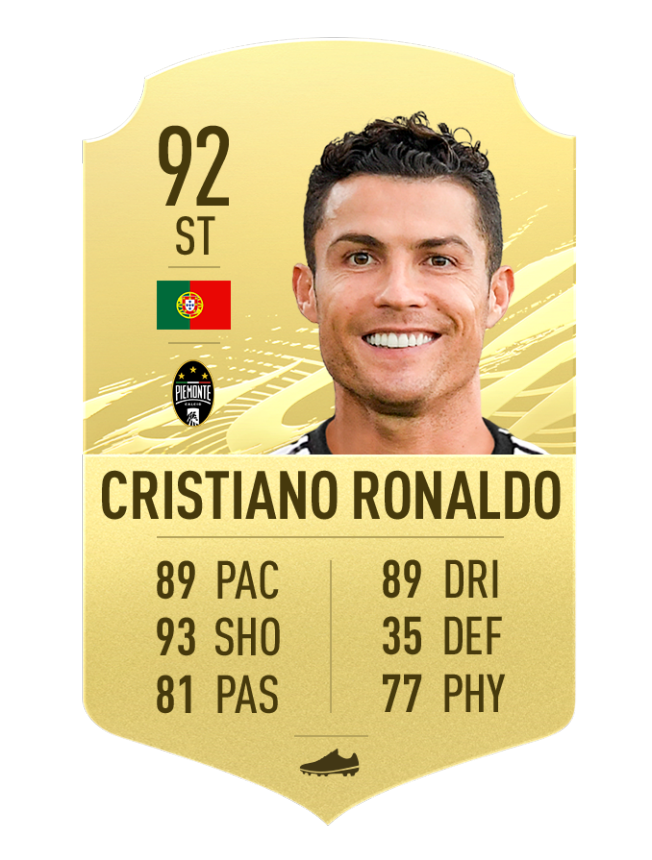
\includegraphics[scale=0.15]{grafiken/Ronaldo}
\caption{Darstellung einer FUT Karte inklusive relevanter Werte am Beispiel Cristiano Ronaldo\\ Quelle: https://www.ea.com/de-de/games/fifa/fifa-21/news/fifa-21-player-ratings-best-strikers-st-cf}
\label{Ronaldo}
\end{wrapfigure}

Bei der dritten Zielgruppe, den Sportwissenschaftlern ist von genügend Vorwissen bezüglich der Daten sowie aller Visualisierungstechniken auszugehen. Bei ihnen stellt sich allerdings noch immer die Frage, welchen Mehrwert ihnen die Visualisierungstechniken bieten können. Beim Baumdiagramm ist dabei von keinem Nutzen auszugehen. Scatterplot und parallele Koordinaten könnten, nach Analyse der Daten auf Realitätsnähe, dazu genutzt werden mögliche Fragestellungen zu beantworten. Weiterhin ist zu sagen, dass dieser Zielgruppe vermutlich nur Erkenntnisse über Trends innerhalb des Datensatzes behilflich sein werden, nicht aber Informationen über spezifische Fussballer.\\

\subsection{Überblick und Beiträge}
%In diesem Abschnitt geben sie einen kurzen Überblick über die Daten und verwendeten Visualisierungen. Dann benennen sie die Beiträge ihres Projekts. Diese Beiträge müssen sie in den hinteren Teilen des Berichts genauer ausführen und belegen.

%\textbf{Sehr kurze Beschreibung der Daten, der Drei Techniken und Beiträge des Projekts(Mehrwert der Visualisierungstechniken)} 


Bei den Daten handelt es sich um einen Datensatz des Fussball Videospiels Fifa 21 dieser enthält Daten zu über 16000 Fussballern. In diesen enthalten sind neben Variablen wie Name, Verein und Alter auch ein ungefähr nach der Qualität des Fussballers festgelegtes Rating sowie Bewertungen der fussballerischen Fähigkeiten (Schießen, Passen, Dribbling, Verteidigen, Geschwindigkeit, Physis, etc.)\\

Die erste verwendete Visualisierungstechnik ist der Scatterplot, dieser ist gut dazu geeignet zwei Variablen der Fussballer zu vergleichen. Bspw. könnte untersucht werden ob ein Fussballer entsprechend seines Könnens (Rating) verdient (Wage). Für Spieler des Karrieremodus können gerade solche Informationen relevant sein, da so Spieler gefunden werden können, die besser spielen als ihr Gehalt es vermuten lassen würde oder solche die zu teuer für ihr können sind.\\

Bei der zweiten verwendeten Visualisierungstechnik handelt es sich um Parallele Koordinaten. Diese, im Vergleich zum Scatterplot, etwas fortgeschrittene Technik eignet sich um mehr als zwei Werte miteinander zu vergleichen. Ihr Einsatz bietet sich daher an um Werte eines Fussballers in den Attributen: Schießen, Passen, Dribbling, Verteidigen, Geschwindigkeit oder Physis miteinander zu vergleichen und dies vorher nach der Position des Fussballers zu Filtern um zu untersuchen ob sich ein Spieler anhand seiner Attribute dafür eignet auf dieser Position zu spielen. (Bsp. ein Stürmer benötigt vor allem Geschwindigkeit, Schießen und Dribbling, ein Verteidiger hingegen Verteidigen, Physis und Geschwindigkeit).
Diese Technik könnte besonders für Spieler des FUT Modus relevant sein, da sich so die besten Spieler für den kompetetiven Online-Modus finden lassen.\\

Die dritte Visualisierungstechnik ist die Darstellung als Baumdiagramm. durch sie werden Spieler ihren Teams und diese ihren jeweiligen Ligen zugeordnet. Da es im FUT Modus ein Chemie System gibt indem ein Team nur gut zusammenspielen kann wenn Spieler einer Liga oder eines Teams entstammen kann ein Nutzer der Visualisierung mit Hilfe dieser ein Team aus einer spezifischen Liga zusammen bauen und nach jeder einzelnen Position filtern\cite{heib_fifa_2021}.



Als dritte und letzte Technik habe ich die Baumdarstellung ausgewählt um sichtbar zu machen welche Fussballliga Europas im Durchschnitt die besten Spieler hat. Deswegen ist dies für X interessant.\\

\section{Daten}
%Beschreiben Sie vorhandenen Daten. Gehen sie kritisch darauf ein, in wie weit sich die Daten für die Bearbeitung der Fragestellungen und dem Erreichen von Lösungen für die oben beschriebene Zielgruppen eignen. Haben sie die Daten sinnvoll mit weiteren Datenquellen ergänzt? Wenn ja, wie?

%\textbf{Beschreibung der gegebenen Daten, Sind sie zur Beantwortung der Fragestellungen geeignet? Welche zusätzlichen Daten wurden genutzt} 

Grundsätzlich eignen sich die Daten gut um die gewünschten Fragestellungen beantworten zu können, jedoch enthält der Grunddatensatz einige Felder, die für die Visualisierung nicht nötig sind, deswegen wurde der Datensatz in der Vorvorarbeitung noch verkleinert (Siehe \ref{Datenvorverarbeitung}). Außerdem ist der Datensatz sehr groß, was gerade bei Scatterplot und parallelen Koordinaten zu Unübersichtlichkeit führen kann wenn der ganze Datensatz angezeigt wird, deswegen wurde sich bei diesen Visualisierungen dazu entschieden nach zusätzliche Filterfunktionalitäten einzubauen um dies so übersichtlicher zu gestalten. Da Datenwerte wie Größe, Alter und Rating der Spieler diskret sind, ist entschieden worden die Opazität der Punkte zu verringern, so ist zu erkennen an welchen Stellen sich mehrere Spieler überlagern. Da ab einer bestimmten Anzahl an Spielern die maximale Opazität erreicht ist und eine geringere Opazität pro Punkt einzelne Punkte fast unsichtbar machen würde, wird im Scatterplot beim hovern über einem Punkt angezeigt wie viele Spieler die genau gleichen  X und Y Werte aufweisen.

\subsection{Technische Bereitstellung der Daten}
%Wie sind die Daten zugänglich? Welche Formate werden genutzt. Gibt es Besonderheiten beim Lesen der Formate?
Die Daten sind in einem privaten Github gehostet\footnote{\url{https://github.com/JohannesLange/Visualisierung_FIFA19/tree/master}}. Dort liegen die Daten der drei Visualisierungen jeweils als \textit{.csv} vor. Die verwendeten Variablen sowie die Anzahl an Fussballern wurden jeweils der Visualisierungstechnik entsprechend angepasst um den Datensatz so klein wie möglich zu halten.

Auch die Daten der Visualisierung als Baumdiagramm liegen als \textit{.csv} vor und werden erst im Programm zu einer \textit{.json} encoded und dann wieder zu einem Baumdiagramm decoded. So liegen die Daten nicht starr als \textit{.json} vor und können innerhalb des Programms vorgefiltert werden. Da der Datensatz keine Daten bezüglich der Fussballligen, in denen die Vereine spielen, enthält, sind diese manuell eingefügt worden.






\subsection{\label{Datenvorverarbeitung}Datenvorverarbeitung}
%Welche Datenvorverarbeitungsschritte sind notwendig? Beschreiben Sie die einzelnen Schritte und begründen sie sie, z.B. warum werden manche Daten weggelassen, über welche Mengen werden Durchschnitte berechnet, warum sind die so berechneten Werte aussagekräftiger als andere Werte. 

Der Datensatz besteht aus Daten von ca. 17000 einzelnen Fussballern, jeder dieser hat 107 einzelne Variablen. Da diese nicht alle relevant für die Visualisierungen sind und ein kleinerer Datensatz die Visualisierung beschleunigt, sind nur die relevanten Variablen ausgewählt worden. Weiterhin unterscheiden sich die Variablen auch zwischen den verschiedenen Visualisierungstechniken. Aus diesem Grund existieren verschieden gefilterte Datensätze für jede Visualisierung.

Die Vorverarbeitung der Daten ist in \textit{R} durchgeführt worden. Das genutzte Skript (\textit{RDataPreprocessing.r}) liegt im Github vor.
Im ersten Schritt des preprocessings sind \textit{NA} Werte aus dem Datensatz entfernt worden.
Außerdem ist der Wert \textit{Height} von Fuß und Inch in Zentimeter umgewandelt worden um so eine Schreibweise ohne nicht-numerische Zeichen zu erhalten (Bsp.: \textit{6''2} wird zu \textit{188}). Weiterhin ist beim Wert \textit{Weight} die Beschriftung \textit{lbs} entfernt worden um den Wert so als \textit{Integer} für den csv-Decoder von elm erkennbar zu machen.
Gleiches ist für die Werte \textit{Wage} und \textit{Value} getan worden. Bei diesen Werten ist die Umwandlung allerdings komplexer, da die Zahlen mit \textit{M} für Millionen und \textit{K} für Tausend abgekürzt sind.
Diese Werte sind in Tausend im finalen Datensatz enthalten. Werte mit \textit{M} sind also mit 1000 multipliziert worden, Werte mit \textit{K} sind entsprechend unverändert geblieben und Werte ohne Buchstaben sind durch 1000 geteilt worden (Bsp.: \textit{1.1M} ist zu \textit{1100} geworden, \textit{90K} zu \textit{90} und \textit{900} zu \textit{0.9}).
Nach dem anpassen dieser Werte können die für \textit{Scatterplot} und \textit{Parallele Koordinaten} relevanten Werte in einem neuen \textit{Data.frame} gespeichert und als \textit{.csv} wieder exportiert werden.  


Der vorhandene Datensatz ist aus zwei verschiedenen Gründen gekürzt worden, zum einen ist die Darstellung durch die Größe des Datensatzes erheblich verlangsamt worden und zum anderen enthält der Datensatz Fussballer für die nicht alle Werte enthalten sind.

Für die Darstellung des Baumdiagramms wurde sich auf die vier größten europäischen Fussballligen (Premier League, Bundesliga, La Liga und Serie A) konzentriert. Deswegen enthält der Datensatz für diese Visualisierungstechnik nur Daten von Spielern, deren Team Teil einer dieser Ligen ist.

Im Git Repository sind unter dem Ordner \textit{data} der ursprüngliche unveränderte Datensatz (\textit{fifa21\_male2.csv}) sowie die veränderten Datensätze (.....) zu finden.

\section{Visualisierungen}
Der gegebene Datensatz wird auf drei verschiedene Arten visualisiert.
Die erste Visualisierung ist ein Scatterplot. Mit diesem können zwei verschiedene Attribute des Datensatzes vom Nutzer freigewählt werden und die Spieler anhand dieser miteinander verglichen werden.\\
Bei der zweiten Visualisierungsform handelt es sich um parallele Koordinaten, diese erlauben im Vergleich zum Scatterplot den Vergleich von mehr als zwei Attributen, sind aber vergleichsweise unübersichtlicher. Weiterhin müssen Nutzer deutlich bewanderter sein um sie interpretieren zu können, da Zusammenhänge nicht benachbarter Attribute kaum erkenntlich sind und vom Nutzer erwartet wird dieser nach Rechts und Links zu verschieben.\\
Die dritte Visualisierung ist ein explizites Baumdiagramm. Mit diesem kann die Struktur der Fussballligen Europas dargestellt werden. Dabei können Nutzer die Liga auswählen und die Spieler nach ihren Positionen filtern.


 Da der Datensatz sehr groß ist können die Spieler nach Verein und Nationalität noch zusätzlich gefiltert werden. Da es trotz dessen noch häufig Überschneidungen der Daten gibt, bspw. bei Alter und Overall der Spieler existiert eine Funktion, die anzeigt wie viele Spieler genau diese Werte aufweisen. Weiterhin sind die angezeigten Punkte teilweise durchsichtig. Dadurch können Überschneidungen der Punkte auch durch deren Opazität erkannt werden.

\subsection{Analyse der Anwendungsaufgaben}
%Analysieren sie die konkreten Anwendungsaufgaben. Welche Visualisierungen helfen den Personen, die die Software verwenden, sinnvolle mentale Modelle aufzubauen. Sind diese mentalen Modelle für sie notwendig, um die Aufgaben lösen zu können?

\textbf{Wie hilft Scatterplot/Parallele Koordinaten/Baumdiagramm die genannten Problemstellungen zu beantworten?}
\subsection{Anforderungen an die Visualisierungen}
%Leiten sie Anforderungen an das Design der Visualisierungen ab, die sich durch ihre Analyse des Zielproblems ergeben.
\textbf{Wie muss die Visualisierung designed werden um das Zielproblem gut beantworten zu können?}
\subsection{Präsentation der Visualisierungen}
%Präsentieren sie die visuelle Abbildungen und Kodierungen der Daten und Interaktionsmöglichkeiten. 
%Sie müssen  begründen, warum und wiegut ihre Designentscheidungen die erstellten Anforderungen erfüllen. 
%Weiterhin müssen sie begründen, warum die gewählte visuelle Kodierung der Daten für das zulösenden Problem passend ist. 
%Typische Argumente würden hier auf Wahrnehmungsprinzipien und Theorie über Informationsvisualisierung verweisen. 
%Die besten Begründungen diskutieren explizit die konkrete Auswahl der Visualisierungen im Kontext von mehreren verschiedenen Alternativen. Diskutieren sie die Expressivität und die Effektivität der einzelnen Visualisierungen. 

%Die eben beschriebenen Präsentationen und Begründungen sollen für jede der drei folgenden Visualisierungen durchgeführt werden. 

\textbf{Visualisierungstechniken vorstellen, Interaktivität zeigen, Designentscheidungen begründen(Erfüllen diese die Anforderungen?), Diskutieren wieso nicht andere Techniken verwendet wurden(Expressivität und Effektivität).}
\subsubsection{Visualisierung Eins}

\begin{figure}[h]
\centering
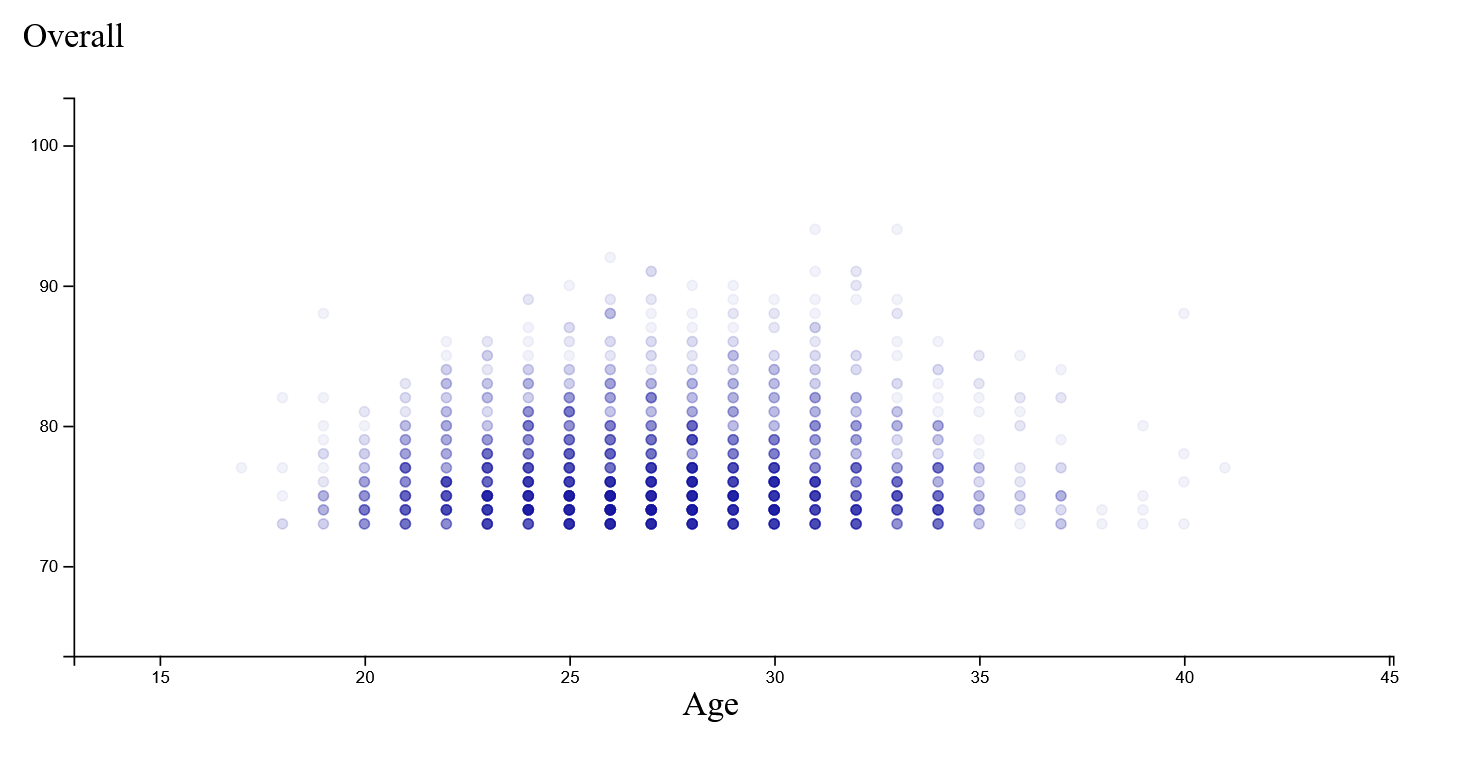
\includegraphics[scale=0.4]{grafiken/Scatterplot1}
\caption{Darstellung des Scatterplots\\ Quelle: eigene Darstellung}
\end{figure}


\subsubsection{Visualisierung Zwei}

\begin{figure}[h]
\centering
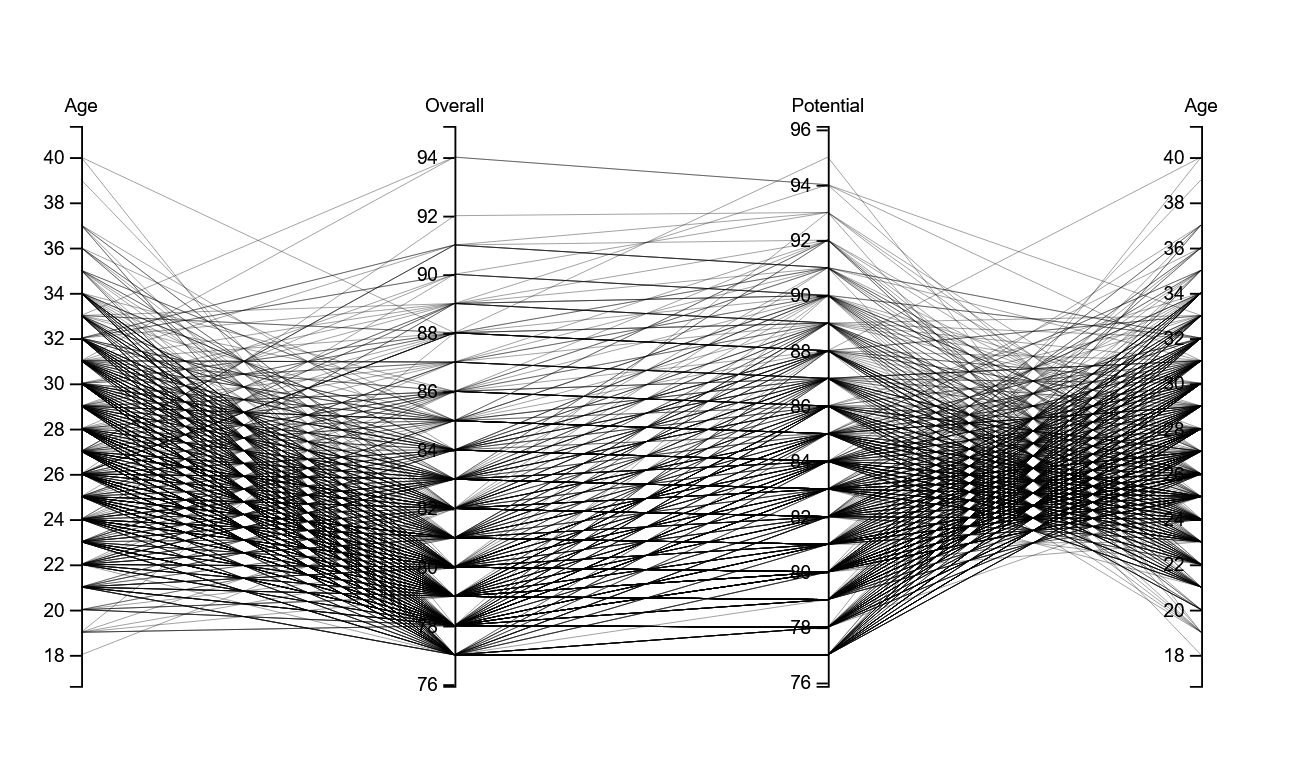
\includegraphics[scale=0.4]{grafiken/ParalleleKoordinaten1}
\caption{Darstellung der Parallelen Koordinaten\\ Quelle: Eigene Darstellung}
\end{figure}






\subsubsection{Visualisierung Drei}
\begin{figure}[h]
\centering
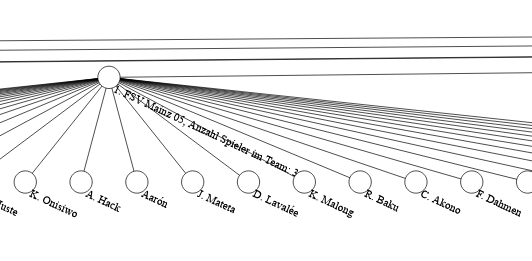
\includegraphics[scale=0.4]{grafiken/BaumDiagram1}
\caption{Ausschnitt aus Baumdarstellung\\ Quelle: Eigene Darstellung}
\end{figure}


\subsection{Interaktion}
%Erklären sie die möglichen Interaktionen mit den einzelnen Visualisierungen und die möglichen Verknüpfungen zwischen ihnen. Begründen Sie warum die konkreten Interaktionen umgesetzt wurden und welche Zwecke für die Anwenderinnen mit ihnen unterstützt werden. Begründen sie ebenfalls warum sie andere Interaktionsmöglichkeiten nicht umgesetzt haben. 

\textbf{Interaktionen in den Visualisierungen(möglicherweise Interaktion zwischen den Techniken), Warum genau diese Techniken, welche Zwecke erfüllen sie für die Anwender, Warum wurden andere nicht umgesetzt}

\section{Implementierung}
%Beschreiben Sie die Implementierung ihrer Visualisierungsanwendung in Elm. Stellen die Gliederung ihres Quellcodes vor. Haben Sie verschiedene Elm-Module erstellt. Was war aufwändig umzusetzen, was ließ sich mit dem vorhanden Code aus den Übungen relativ einfach umsetzen? 

%Wie sieht die Elm-Datenstruktur für das Model aus, in dem die verschiedenen Zustände der Interaktion gespeichert werden können.

\textbf{Wie ist der Quellcode gegliedert, was lies sich aus den Übungen übernehmen, Wie sieht die Datenstruktur des Modells aus -> in dem verschiedene Zustände der Interaktion gespeichert wurden (Success record)}

\section{Anwendungsfälle}
%Präsentieren sie für jede der drei Visualisierungen einen sinnvollen Anwendungsfall in dem ein bestimmter Fakt, ein Muster oder die Abwesenheit eines Musters visuell festgestellt wird. Begründen sie warum dieser Anwendungsfall wichtig für die Zielgruppe der Anwenderinnen ist. Diskutieren sie weiterhin, ob die oben beschriebene Information auch mit anderen Visualisierungstechniken hätte gefunden werden können. Falls dies möglich wäre, vergleichen sie die den Aufwand und die Schwierigkeiten ihres Ansatzes und der Alternativen. 

\textbf{Spezifischen Anwendungsfall für Nutzergruppen vorstellen, der an Hand der Visualisierungstechniken visuell erkennbar ist, wäre dies auch mit anderen Techniken möglich gewesen? Aufwand mit anderen Techniken vergleichen}
\subsection{Anwendung Visualisierung Eins}



\subsection{Anwendung Visualisierung Zwei}


\subsection{Anwendung Visualisierung Drei}

\section{Verwandte Arbeiten}
%Führen sie eine kurze Literatursuche in der wissenschaftlichen Literatur zu Informationsvisualisierung und Visual Analytics nach ähnlichen Anwendungen durch. Diskutieren sie mindestens zwei Artikel. Stellen sie Gemeinsamkeiten und Unterschiede dar.
\textbf{Zwei Artikel mit ähnlichen Zielen diskutieren}
\section{Zusammenfassung und Ausblick}
%Fassen sie die Beiträge ihre Visualisierungsanwendung zusammen. Wo bietet sie für die Personen der Zielgruppe einen echten Mehrwert.

\textbf{Beiträge der Anwendung, welcher Mehrwert für Zielgruppe entsteht, mögliche Erweiterungen(Visualisierungen oder Daten)}
%Was wären mögliche sinnvolle Erweiterungen, entweder auf der Ebene der Visualisierungen und/oder auf der Datenebene?

\newpage

\pagenumbering{Roman}
\setcounter{page}{4}
\section*{Anhang: Git-Historie}
Das die Commits von zwei verschiedenen Accounts stammen ist zu entschuldigen. Die Anmeldung in der GIT GUI von Windows ist unabsichtlich mit einem anderen Account vorgenommen worden und erst später bemerkt worden.

\begin{verbatim}
* ba194f5 (HEAD -> master, origin/master) (Writing Chapter 2, 2021-09-09)
* a32805e (Changes to html testsite, 2021-09-09)
* fcfa8fa (Updates to Scatterplot, 2021-09-08)
* 9f41152 (Added additional filterfunctionality to parallelCoordinates, 2021-09-08)
* 130d43d (Updated Readme.md, 2021-09-08)
* bcb2233 (changes to spData.csv reagrding encoding, 2021-09-08)
* 14007ce (Added filter functionality to parallel Coordinates, 2021-09-08)
* b373216 (deleted unused datasets, 2021-09-08)
* 75f726f (started writing chapter preprocessing, 2021-09-08)
* a2207bf (Renaming of elm files and Creation of elm files with smaller csv files, 2021-09-08)
* a2e9801 (fixed error in index.html, 2021-09-08)
* da0991c (Included new html file for parallel COordinates, 2021-09-08)
* 9f20f40 (Updated RDataPreprocessing file, 2021-09-08)
* c72d4a2 (Updated spData and spData2000 with value and wage, 2021-09-08)
* e46740a (test changes in spData.csv, 2021-09-08)
* 956bf26 (test update spDate, 2021-09-08)
* 379c0de (updated spData again, 2021-09-08)
* 477c43a (Updated spData.csv with wage and value data, 2021-09-08)
* 3c200e1 (Updated Baumdata.csv with Premier League Data, 2021-09-07)
* 3af31ee (Updated Baum csv data with serie a players, 2021-09-07)
* 1e66fcd (Development of Filterfunction for Players Positions in Treediagram, 2021-09-07)
* 1cfd18f (Updated Baumdata.csv, 2021-09-07)
* f5adf5f (reworking of 1.1, 2021-09-07)
* 1bd9293 (Creation of Tree.html, 2021-09-07)
* b04c990 (Created index.html for github pages, 2021-09-07)
* ebfba7f (Updated bibtex file, 2021-09-07)
* c6240a4 (First try of preprocessing parallel coordinates data, 2021-09-06)
* 43ba73b (Added highlighting and Player info on hover, 2021-09-06)
* 447a93e (changed additional errors in baumData.csv reagrding laLiga players, 2021-09-06)
* 30992b9 (fixed errors in LaLiga club names, 2021-09-06)
* 3a8659a (Updated Baumdata.csv with laliga clubs, 2021-09-06)
* 7a98e59 (Started writing preprocessing file in R, 2021-09-06)
* d4b3df2 (Changed error in Baumdata regarding multiple club names, 2021-09-06)
* c825fef (Created test csv Data for Baumdiagram, 2021-09-06)
* 79150e1 (Implementation of Filter function in the Scatterplot as well as changes to the selections, 2021-09-06)
* d3bc365 (-Created Fifa 21 Scatterplot Data, reduced to 2000 Players, 2021-09-05)
* 605e204 (Added preliminary Scatterplot Data from Fifa 21, 2021-09-05)
* cce366d (-Reorganization and inclusion of placeholder images, 2021-09-05)
* a6328bf (Added full csv of fifa 21 data to gitignore, 2021-09-05)
* abbce42 (started writing chapter 2.2, 2021-09-05)
* 1bcf321 (-Reorganized git 2 deleting additional, unused files, 2021-09-05)
* 0017063 (-Reorganized git, 2021-09-05)
* e5ebc82 (Updated Readme.me, 2021-09-05)
* 93b8a97 (-Started writing Chapter 2.1, 2021-09-05)
* 4477dba (Started writing chapter 1.3, 2021-09-05)
* 7be9390 (Started writing Chapter Zielgruppen, 2021-09-04)
* 2386040 (Reduced size of csv for testing purposes, 2021-08-22)
* 5d98177 (Added Nationality to CSV, 2021-08-22)
* a395085 (Added smaller CSV tree file, 2021-08-15)
* 4fa41ce (New Test CSV File for ElmTreeMap, 2021-08-15)
* 5952879 (Added .json file and Excercise tree visualization code to start implementing tree visualization, 2021-08-14)
* 1295900 (-Changed name of tex and pdf file and added new folder AbgabeOrdnerLatex, 2021-08-13)
* 5c1747d (-Changed gitignore to new Latex files, 2021-08-13)
* 9443014 (Kapitel 2 Daten Version 0.1, 2021-08-12)
* f673cd6 (-Grundlagen des Projektberichts, 2021-08-12)
* cd852b2 (TXT statt csv, 2021-08-12)
* 9c07724 (-Added smaller CSV with 1000 lines, 2021-08-12)
* a441b52 (-csv, 2021-08-12)
* 2f7fbe0 (-csv, 2021-08-12)
* 8ac06b8 (-minor fixes csv, 2021-08-12)
* cc9cede (Prefiltering of Data, 2021-08-12)
* eb68618 (Testing error with height, 2021-08-12)
* 95935c0 (Testing Height in Metres instead of CM, 2021-08-12)
* ef3a227 (Rounded Height, 2021-08-12)
* cb4c956 (Reduced CSV file, 2021-08-12)
* f0e6cae (Added Interactivity to parallel Coordinates, 2021-08-11)
* 9ee66e1 (Added Parallele Koordinaten Grundfunktionalität, 2021-08-11)
* eb4f173 (-Added Git Folder structure, 2021-08-11)
* 7d09347 (Added changeablity to the data, 2021-08-10)
* 07422d2 (Extended number of encodeable variables for the Scatterplot, 2021-08-06)
* a6fd816 (-Added possibility to change variables, 2021-08-03)
* f0f68ea (-Updated PointName -Started writing Paper, 2021-08-03)
* adfd7a6 (-First working Scatterplot, 2021-08-03)
* c4f4b5f (-Scatterplot first tries, 2021-08-03)
* f9af25c (-Commiting new files, 2021-07-30)
* 4618601 (Upload pdf, 2021-07-07)
* d267f3d (-deleted Latex files, 2021-07-07)
*   65fd4fd (Merge branch 'master' of https://github.com/Blauekuh/Visualisierung_FIFA19.git, 2021-07-07)
|\
| * 68629b2 (Update .gitignore, 2021-07-07)
* | 7aaf7f3 (Latex File created, 2021-07-07)
|/
* be4234d (-Added gitignore, 2021-07-05)
* 546ae0e (Upload CSV Dataset for Fifa 19, 2021-06-17)
* c640421 (Commit of first test elm file, 2021-06-16)
* fcdc3ad (origin/main, origin/Development) (Initial commit, 2021-06-16)
\end{verbatim}



\printbibliography

\end{document}

